% Auto-filled draft using your uploaded summaries (front/side).
% Compile: pdflatex main.tex ; bibtex main ; pdflatex main.tex ; pdflatex main.tex
\documentclass[conference]{IEEEtran}
\IEEEoverridecommandlockouts

\usepackage{cite}
\usepackage{amsmath,amssymb}
\usepackage{graphicx}
\usepackage{booktabs}
\usepackage{multirow}
\usepackage{xcolor}
\usepackage{url}
\usepackage{array}
\usepackage{tikz}
\usetikzlibrary{
    arrows.meta,
    positioning,
    fit,
    backgrounds
}


\begin{document}

\title{AI Virtual Coach with Multi-Stage Pipelines for Exercise Recognition and Pose-Based Assessment\thanks{This work involved human subjects in its research. The author(s) confirm(s) that all human subject research procedures and protocols are exempt from review board approval. Participation was voluntary, verbal informed agreement was obtained from all volunteers, and all collected data were anonymized using numerical identifiers to preserve participant privacy.}}

\author{
\IEEEauthorblockN{Anonymous Author(s)}
\IEEEauthorblockA{Paper under double-blind review}
}

\maketitle

\begin{abstract}
We present an AI Virtual Coach composed of two main models: (i) Exercise Recognition, and (ii) Exercise Assessment.
The assessment module performs aspect-level scoring for 15 resistance-training exercises using temporal pose sequences extracted from RGB video via MediaPipe, repetition segmentation, and a compact temporal CNN regressor.
We evaluate on a small dataset of 51 volunteers (10 female, 41 male), captured simultaneously in front and side views using mobile phones.
Each exercise includes 6--13 volunteers (after alignment), and each volunteer is rated on five aspects (0--10) by two coaches.
We use a reliability-weighted label, a subject-disjoint protocol, and 10 randomized runs per exercise per view with best-checkpoint selection.
\end{abstract}

\begin{IEEEkeywords}
Virtual coach, pose estimation, exercise recognition, action quality assessment, exercise assessment, temporal CNN, rep segmentation, MediaPipe
\end{IEEEkeywords}

\section{Introduction}
%% TODO (you): 1–2 paragraphs:
%% - Why virtual coaching matters, constraints of consumer RGB/mobile
%% - Your 3-module pipeline and what each part enables
%% - Mention small dataset challenge and how you handle it

\textbf{Contributions.} We contribute:
\begin{itemize}
  \item A practical modular virtual-coach pipeline (exercise recognition, assessment, coaching agent).
  \item A pose-based assessment method that segments repetitions, aggregates multiple reps per volunteer, and predicts five aspect scores on a 0–10 scale.
  \item A subject-disjoint multi-run evaluation protocol for small datasets, saving the best model per exercise and view.
\end{itemize}

\section{Related Work}
\subsection{Action Quality Assessment}
FLEX introduces a large-scale multimodal, multiview dataset and benchmarks for action quality assessment.
CoRe proposes group-aware contrastive regression for learning AQA from comparisons.
\subsection{Pose-Based Motion Modeling}
MediaPipe/BlazePose enables real-time pose landmark extraction from RGB video.
Gait-ViT demonstrates the effectiveness of Transformer-based temporal modeling on gait sequences.
\subsection{What Makes Our Work Different}
Most AQA work targets broad action categories and relies on large-scale training data, while our setting focuses on 15 gym exercises with a constrained dataset (51 volunteers) and two consumer-camera views.
Unlike single-score AQA, we predict five \emph{aspect-level} scores per exercise (0--10), and explicitly model repetitions via segmentation and aggregation so multi-rep videos can be graded fairly.


\section{Methods}
This section describes our data collection process, pose feature extraction pipeline, and the proposed models for exercise recognition and exercise assessment.

\subsection{Data Collection}

\subsubsection{Participants}
The dataset was collected from 51 recreationally active volunteers, including 41 males (80.4\%) and 10 females (19.6\%). Participants ranged in age from 15 to 29 years (mean: 21.3 years), with the majority belonging to the 21--22 age group.

Participant heights ranged from 158 cm to 190 cm (mean: 174.2 cm), while body weights ranged from 52 kg to 110 kg (mean: 77.5 kg). Corresponding Body Mass Index (BMI) values ranged approximately from 18 to 37, with an average BMI of 24.7.

All participants reported no current musculoskeletal injuries at the time of recording.


\subsubsection{Exercise Set}
The dataset includes recordings of 15 resistance training exercises covering both upper- and lower-body movements:

\begin{itemize}
    \item Dumbbell Shoulder Press
    \item Hammer Curls
    \item Standing Dumbbell Front Raises
    \item Lateral Raises
    \item Bulgarian Split Squat
    \item EZ-Bar Curls
    \item Incline Dumbbell Bench Press
    \item Overhead Triceps Extension
    \item Shrugs
    \item Weighted Squats
    \item Seated Biceps Curls
    \item Triceps Kickbacks
    \item Rows
    \item Deadlift
    \item Calf Raises
\end{itemize}

Overall, the dataset contains a larger variety of upper-body exercise types than lower-body exercise types. However, the number of volunteers contributing to each exercise was approximately comparable across upper- and lower-body movements, reflecting natural participation during the recording sessions.


\subsubsection{Recording Setup and Protocol}
All recordings were conducted indoors at multiple local gym facilities in Egypt. Videos were captured using a smartphone camera at a resolution of 1080~$\times$~1920 pixels and a frame rate of 30 frames per second, in landscape orientation. Lighting conditions varied across sessions, resulting in mixed indoor illumination.

Camera height and distance were not strictly fixed and varied depending on the exercise, though recordings generally captured either the full body or were positioned at approximately waist level. Each video corresponds to a single exercise set lasting approximately 30 to 60 seconds and containing 8 to 12\textbf{ }repetitions, recorded as a continuous sequence.

Participants performed exercises using self-selected weights to emulate realistic training conditions. Exercise execution was performed naturally, allowing for intra- and inter-subject variability in movement quality, which is essential for form assessment modeling.


\subsubsection{Viewpoint Acquisition}
To capture complementary kinematic information, each exercise was recorded from two viewpoints:
\begin{itemize}
    \item Front view
    \item Side view
\end{itemize}

A total of 154 videos per viewpoint were recorded, resulting in 308 videos overall. Each video was segmented into repetition-level clips, where each clip corresponds to a single exercise repetition. Viewpoints were manually labeled during preprocessing.


\subsubsection{Expert Annotation}
Each recorded exercise set was annotated by two certified fitness coaches using  reliability-weighted label $y=0.25y_{C1}+0.75y_{C2}$ based on a joint review of the corresponding front-view and side-view videos. Annotations were performed at the video (set) level, rather than at the individual repetition level.

For each exercise, coaches evaluated five predefined biomechanical aspects specific to that movement, such as joint alignment, range of motion, stability, and movement control. These criteria were defined in advance for each exercise to ensure consistency across annotations.

The resulting annotation scores represent an overall quality assessment of the exercise set and were used as supervisory signals for training and evaluating the proposed exercise assessment model. Repetition-level clips extracted from each video inherit the corresponding set-level annotation.


\subsubsection{Dataset Limitations}
The dataset exhibits a gender imbalance, with a higher proportion of male participants, as well as a limited number of lower-body exercise samples. These limitations are primarily due to cultural and logistical constraints during data collection. Nevertheless, the dataset captures substantial inter-subject variability and realistic execution patterns, making it suitable for evaluating virtual coaching and exercise assessment systems.


\subsection{System Overview}

Figure~\ref{fig:pipeline} illustrates the end-to-end pipeline of our AI Virtual Coach. The system processes a single-view RGB video (either front or side) and produces structured textual feedback through four sequential stages.

\textbf{Stage 1: Pose Estimation and Feature Extraction.}
Given an input video, we extract 3D pose landmarks for each frame using MediaPipe Pose Landmarker. The raw landmarks are normalized for scale and translation invariance (Section~\ref{sec:pose_gen}), and nine biomechanical joint angles are computed per frame. The resulting temporal sequence is resampled to a fixed length of $T=50$ timesteps, yielding a feature tensor of shape $(50, 9)$ per repetition.

\textbf{Stage 2: Exercise Recognition.}
The temporal pose features are passed to an MLP classifier that identifies which of the 15 supported exercises is being performed. The predicted exercise class determines which exercise-specific assessment model to invoke, enabling specialized evaluation tailored to each movement's biomechanics.

\textbf{Stage 3: Per-Repetition Assessment.}
Based on the recognized exercise, the corresponding assessment model (one of 15 trained separately per exercise and view) evaluates each detected repetition. Rather than outputting a single aggregated score, the model produces \emph{per-repetition} scores for five exercise-specific aspects (e.g., joint alignment, range of motion, tempo, stability). This fine-grained output enables downstream analysis of form consistency and fatigue patterns across the set.

\textbf{Stage 4: Coaching Agent.}
The per-rep assessment scores, along with exercise-specific evaluation criteria, are passed to a stateful coaching agent implemented using LangGraph. The agent performs rule-based trend analysis to detect fatigue (by comparing early vs.\ late reps), computes a consistency score (inverse of score variance), and identifies the strongest and weakest aspects. These analytical results, together with the detailed per-rep breakdown, are then passed to a large language model (Google Gemini) that generates personalized, actionable coaching feedback in natural language. The final output includes aggregated scores, trend indicators, fatigue warnings, and a conversational feedback summary suitable for display in a mobile application.

\begin{figure*}[t]
\centering
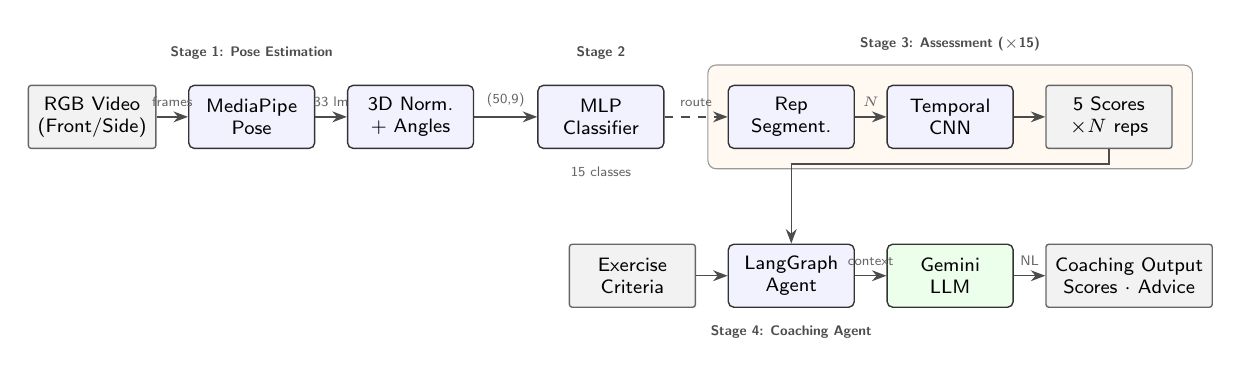
\begin{tikzpicture}[
    font=\sffamily\scriptsize,
    node distance=4mm,
    box/.style={
        rectangle,
        rounded corners=2pt,
        draw=black!80,
        fill=blue!5,
        line width=0.5pt,
        align=center,
        minimum height=8mm,
        minimum width=16mm
    },
    data/.style={
        rectangle,
        rounded corners=1pt,
        draw=black!60,
        fill=gray!10,
        line width=0.5pt,
        align=center,
        minimum height=8mm,
        minimum width=16mm
    },
    stage/.style={
        font=\sffamily\tiny\bfseries,
        text=black!70
    },
    annot/.style={
        font=\sffamily\tiny,
        text=black!60
    },
    arrow/.style={->, >=Stealth, line width=0.5pt, black!70},
    dashedarrow/.style={->, >=Stealth, dashed, line width=0.5pt, black!70}
]

% ===== ROW 1: Stages 1-3 =====
\node[data] (rgb) {RGB Video\\(Front/Side)};
\node[box, right=of rgb] (mp) {MediaPipe\\Pose};
\node[box, right=of mp] (norm) {3D Norm.\\+ Angles};
\node[box, right=8mm of norm] (mlp) {MLP\\Classifier};
\node[box, right=8mm of mlp] (rep) {Rep\\Segment.};
\node[box, right=of rep] (cnn) {Temporal\\CNN};
\node[data, right=of cnn] (score) {5 Scores\\$\times N$ reps};

\draw[arrow] (rgb) -- node[annot, above]{frames} (mp);
\draw[arrow] (mp) -- node[annot, above]{33 lm} (norm);
\draw[arrow] (norm) -- node[annot, above]{(50,9)} (mlp);
\draw[dashedarrow] (mlp) -- node[annot, above]{route} (rep);
\draw[arrow] (rep) -- node[annot, above]{$N$} (cnn);
\draw[arrow] (cnn) -- (score);

% Stage labels (row 1)
\node[stage, above=2mm of mp] {Stage 1: Pose Estimation};
\node[stage, above=2mm of mlp] {Stage 2};
\node[annot, below=1mm of mlp] {15 classes};

% Stage 3 bounding box
\begin{scope}[on background layer]
\node[
    draw=black!40,
    rounded corners=3pt,
    line width=0.4pt,
    fill=orange!5,
    fit=(rep)(cnn)(score),
    inner sep=2.5mm,
    label={[stage, above=0.5mm]north:Stage 3: Assessment ($\times$15)}
] {};
\end{scope}

% ===== ROW 2: Stage 4 =====
\node[box, below=12mm of rep] (agent) {LangGraph\\Agent};
\node[data, left=of agent] (crit) {Exercise\\Criteria};
\node[box, right=of agent, fill=green!8] (llm) {Gemini\\LLM};
\node[data, right=of llm, minimum width=20mm] (out) {Coaching Output\\Scores $\cdot$ Advice};

\draw[arrow] (score) -- ++(0,-6mm) -| (agent);
\draw[arrow] (crit) -- (agent);
\draw[arrow] (agent) -- node[annot, above]{context} (llm);
\draw[arrow] (llm) -- node[annot, above]{NL} (out);

\node[stage, below=1mm of agent] {Stage 4: Coaching Agent};

\end{tikzpicture}
\caption{End-to-end pipeline. Stage~1 extracts pose landmarks and joint angles. Stage~2 classifies the exercise (15 classes). Stage~3 segments repetitions and applies exercise-specific temporal CNN models for per-rep aspect scores. Stage~4 uses LangGraph with Gemini LLM for personalized feedback.}
\label{fig:pipeline}
\end{figure*}





\subsection{Pose Data Generation}
\label{sec:pose_gen}

\subsubsection{Pose Landmark Extraction}
For each video frame, 3D human pose landmarks were extracted using the MediaPipe Pose Landmarker Lite model \cite{mediapipe}. The model produces 33 body landmarks per frame, each with $(x, y, z)$ coordinates, where $x$ and $y$ represent normalized image-plane coordinates and $z$ represents depth from the camera plane. Detection and tracking confidence thresholds were set to 0.3. Frames were converted from BGR to RGB color space for MediaPipe compatibility, and a fresh \texttt{PoseLandmarker} instance was created per video to ensure proper timestamp handling in VIDEO mode.

\subsubsection{3D Landmark Normalization}
To achieve scale and translation invariance with respect to camera distance and subject body size, all landmarks were normalized in 3D space using a torso-length-based transformation. First, the pelvis center $\mathbf{p}$ was computed as the midpoint of the left hip (landmark 23) and right hip (landmark 24):
\begin{equation}
\mathbf{p} = \frac{1}{2}(\mathbf{h}_{23} + \mathbf{h}_{24}),
\end{equation}
where $\mathbf{h}_{i} = (x_i, y_i, z_i)$. Similarly, the mid-shoulder point $\mathbf{s}$ was computed as the midpoint of the left shoulder (landmark 11) and right shoulder (landmark 12):
\begin{equation}
\mathbf{s} = \frac{1}{2}(\mathbf{h}_{11} + \mathbf{h}_{12}).
\end{equation}
The torso length $L$ in 3D space was then calculated as:
\begin{equation}
L = \|\mathbf{s} - \mathbf{p}\| = \sqrt{(s_x - p_x)^2 + (s_y - p_y)^2 + (s_z - p_z)^2}.
\end{equation}
Finally, each landmark $\mathbf{h}_i$ was normalized as:
\begin{equation}
\mathbf{h}_i^{\text{norm}} = \frac{\mathbf{h}_i - \mathbf{p}}{L}.
\end{equation}
Frames with invalid torso length ($L < 10^{-6}$) were discarded to ensure numerical stability.

\subsubsection{Joint Angle Computation}
From the normalized 3D landmarks, nine biomechanical joint angles were computed per frame using the 3D dot product formula. For each angle defined by a triplet of landmarks $(a, b, c)$ where $b$ is the joint vertex, the angle $\theta$ was calculated as:
\begin{equation}
\theta = \arccos\left(\frac{\mathbf{v}_1 \cdot \mathbf{v}_2}{\|\mathbf{v}_1\| \|\mathbf{v}_2\|}\right),
\end{equation}
where $\mathbf{v}_1 = \mathbf{h}_a - \mathbf{h}_b$ and $\mathbf{v}_2 = \mathbf{h}_c - \mathbf{h}_b$ are vectors in 3D space. The nine angles extracted were: left and right elbow (landmarks 11-13-15 and 12-14-16), left and right shoulder (13-11-23 and 14-12-24), left and right hip (11-23-25 and 12-24-26), left and right knee (23-25-27 and 24-26-28), and torso lean (computed from mid-shoulder and pelvis alignment).

\subsubsection{Temporal Feature Representation}
For each exercise repetition, the nine joint angle time series were resampled to a fixed temporal length of $T_{\text{fixed}} = 50$ frames using linear interpolation to enable batch processing and model training. Let $\theta_j^{(t)}$ denote the $j$-th angle at original time index $t \in [0, T_{\text{orig}}-1]$. We defined a normalized time axis $\tau \in [0, 1]$ and applied linear interpolation to obtain angle values at target time indices $\tau' \in [0, 1]$ uniformly spaced with $T_{\text{fixed}}$ points. This resampling process produced temporal feature tensors of shape $(N_{\text{reps}}, 50, 9)$, where $N_{\text{reps}}$ is the total number of repetitions across all volunteers and exercises.

Edge cases were handled as follows: sequences with $T_{\text{orig}} = 0$ were filled with zeros, single-frame sequences ($T_{\text{orig}} = 1$) were replicated across all 50 timesteps, and sequences with $T_{\text{orig}} > 1$ underwent standard linear interpolation.

\subsubsection{Tempo Preservation}
Since resampling to a fixed length inherently discards information about exercise execution speed, we explicitly preserved tempo as separate feature arrays. For each repetition, we computed: (i) \textbf{tempo\_duration\_sec}, the FPS-normalized duration in seconds calculated as $D = T_{\text{orig}} / \text{FPS}$, where $\text{FPS}$ is the video frame rate; (ii) \textbf{tempo\_frame\_count}, the total number of frames in the original video; and (iii) \textbf{tempo\_fps}, the original video FPS. These tempo features allow the model to distinguish between fast and slow executions of the same exercise, which is critical for movement quality assessment.

All processed pose data, including temporal angle sequences and tempo metadata, were stored in compressed NumPy archive (NPZ) format with data type \texttt{float32} for use in exercise recognition and assessment tasks.

 

\subsection{Exercise Recognition}
The exercise recognition module classifies 15 resistance training exercises from temporal pose sequences using a multilayer perceptron (MLP). This module processes the temporal features extracted as described in Section~III-B and performs subject-disjoint classification to ensure generalization to unseen individuals.

\subsubsection{Model Architecture}
The temporal pose sequences of shape $(N, 50, 9)$ were flattened into 450-dimensional feature vectors, where each vector represents the concatenated time series of nine joint angles over 50 timesteps. A feedforward neural network with three hidden layers was employed, with layer sizes of 384, 192, and 96 neurons respectively. Each hidden layer was followed by ReLU activation and dropout regularization with a dropout rate of 0.30 to prevent overfitting. The output layer consisted of 15 neurons with softmax activation for multi-class classification.

\subsubsection{Training Protocol}
The model was trained using the Adam optimizer with a learning rate of $8 \times 10^{-5}$ and a batch size of 16. Training was conducted for a maximum of 200 epochs with early stopping monitoring validation loss, using a patience of 50 epochs and restoring the best weights upon convergence. Learning rate reduction on plateau was enabled with a factor of 0.5 and a patience of 15 epochs. The loss function was sparse categorical cross-entropy, and both accuracy and macro-averaged F1 score were monitored during training.

\subsection{Assessment Module}
Our assessment framework converts raw exercise videos into \emph{subject-level} performance scores through four stages: pose-based feature construction, repetition segmentation, repetition-to-subject aggregation, and multi-aspect regression. The full pose preprocessing and temporal feature representation are described in Section~III-B.

\subsubsection{Pose Extraction and Kinematic Feature Construction}
Each frame is processed with MediaPipe to obtain 3D pose landmarks (33 keypoints). As described in Section~III-B, landmarks are normalized in 3D for scale and translation invariance, and a compact set of nine biomechanical joint-angle features is computed per frame. For each detected repetition, the resulting angle time series is resampled to a fixed length of $T=50$ time steps, producing a tensor of shape $(N_{\text{reps}}, 50, 9)$.
Because temporal resampling removes absolute speed information, we preserve repetition tempo as additional metadata (e.g., original frame count and duration in seconds), enabling the model to distinguish fast and slow executions.

\subsubsection{Repetition Segmentation via Exercise/View-Specific Signals}
We segment repetitions directly from the pose stream using a 1D exercise/view-specific ``rep signal'' designed to capture the primary biomechanical cycle of the movement (e.g., wrist/arm elevation for raises and pressing, elbow flexion for curls, hip/knee depth for squats and split squats). The rep signal is temporally smoothed, and repetitions are detected using a robust threshold-based cycle logic (up--down--up or down--up--down) with:
(i) adaptive thresholds (computed from within-video statistics) to handle subject variability,
(ii) hysteresis to prevent rapid state flipping near thresholds, and
(iii) minimum-duration and minimum-separation constraints to avoid double counting due to noise.
This yields a variable number of repetitions $N_{\text{reps}}$ per video.

\subsubsection{Repetition Windowing and Subject-Level Aggregation}
Each detected repetition is represented as a fixed-length temporal window (already resampled to $T=50$) of the nine angle features. A temporal encoder maps each repetition $r$ to an embedding $e_r \in \mathbb{R}^d$.
Since ground-truth annotations are provided at the \emph{set/video} level (not per repetition), we aggregate the repetition embeddings into a single subject-level representation using masked attention pooling to handle variable $N_{\text{reps}}$:
\begin{equation}
\alpha_r = \frac{m_r \exp(a(e_r))}{\sum_k m_k \exp(a(e_k))}, \qquad
e_{\text{subj}} = \sum_r \alpha_r e_r,
\end{equation}
where $a(\cdot)$ is a lightweight scoring network and $m_r \in \{0,1\}$ is a binary mask indicating valid repetitions.

\subsubsection{Temporal CNN Regressor and Training Objective}
We use a compact temporal CNN (1D convolutions over the time axis) to encode each repetition window and produce $e_r$. A shallow prediction head outputs five aspect scores per sample. During training, target labels are normalized to $[0,1]$ and optimized with mean squared error (MSE). At inference, outputs are rescaled to the original 0--10 range.

When two coaches provide scores for a given set, we use a reliability-weighted fusion:
\begin{equation}
y = 0.25\,y_{C1} + 0.75\,y_{C2}.
\end{equation}
We train and evaluate the assessment model separately per exercise and per view (front/side) under subject-disjoint splits, and report MAE on the 0--10 scale.


\section{Experimental Setup}

\subsection{Data Splitting Protocol}
To ensure robust performance evaluation and prevent subject leakage, we employed a \textbf{subject-disjoint} stratified splitting strategy where each volunteer appeared in exactly one of the train (55\%), validation (15\%), or test (30\%) sets. Stratification guarantees that all 15 exercise classes are represented in each split, which is critical especially in the held-out test set to ensure true generalization for our proposed models.

\subsection{Multi-Run Evaluation}
To account for variance due to random initialization and data splitting, we conducted multiple independent training runs with different random seeds. For exercise recognition, we conducted 30 independent training runs (base seed 42 with incremental offsets). For exercise assessment, we repeat training for 10 randomized runs and select the best checkpoint (lowest MAE) per exercise/view.

\subsection{Evaluation Metrics}
For exercise recognition, both accuracy and macro-averaged F1 score were monitored during training. For exercise assessment, we report Mean Absolute Error (MAE) on the 0--10 scale. In our current implementation, the reported MAE is a macro average computed across all aspects and all test subjects for that run.
%% TODO (recommended): also report per-aspect MAE, and correlation metrics (Pearson/Spearman).


\section{Results and Discussion}

\subsection{Exercise Recognition Results}
Table~\ref{tab:exer_recog_results} summarizes the aggregated performance across 30 runs for both front and side views on the temporal pose data. The side-view model achieved a mean test accuracy of $89.26\% \pm 2.64\%$ and a mean macro-averaged F1 score of $87.74\% \pm 2.88\%$, while the front-view model achieved $76.16\% \pm 4.57\%$ accuracy and $75.08\% \pm 5.07\%$ macro F1. The side view consistently outperformed the front view by approximately 13 percentage points, suggesting that lateral body profiles provide more discriminative pose features for distinguishing between exercises.

\begin{table}[t]
\centering
\caption{Exercise Recognition Results (30 Runs per View)}
\label{tab:exer_recog_results}
\begin{tabular}{llcc}
\toprule
\textbf{View} & \textbf{Metric} & \textbf{Mean $\pm$ Std} & \textbf{Range} \\
\midrule
\multirow{2}{*}{Side} & Accuracy (\%) & $89.26 \pm 2.64$ & $[83.78, 94.90]$ \\
 & Macro F1 (\%) & $87.74 \pm 2.88$ & $[81.16, 93.24]$ \\
\midrule
\multirow{2}{*}{Front} & Accuracy (\%) & $76.16 \pm 4.57$ & $[68.34, 86.38]$ \\
 & Macro F1 (\%) & $75.08 \pm 5.07$ & $[65.70, 86.34]$ \\
\bottomrule
\end{tabular}
\end{table}

Per-class F1 scores for the side view revealed strong performance across most exercises, with several classes achieving F1 scores above 0.95 (Deadlift: 0.962, Rows: 0.960, Seated Biceps Curls: 0.977, Triceps Kickbacks: 0.957, Weighted Squats: 0.955). Classes with lower performance included Overhead Triceps Extension (0.654) and Shrugs (0.590), likely due to subtle biomechanical differences that are difficult to capture from the side view alone. Figures~\ref{fig:confusion_side} and~\ref{fig:confusion_front} present the aggregated normalized confusion matrices for side and front views respectively, averaged across all 30 runs. Both views show strong diagonal dominance, though the front view exhibits more inter-class confusion, particularly among curl variants and raises.

\begin{figure}[t]
\centering
\includegraphics[width=0.48\textwidth]{confusion_matrix_side_temporal.png}
\caption{Aggregated confusion matrix for exercise recognition (side view, mean across 30 runs, normalized). Strong diagonal indicates robust per-class performance.}
\label{fig:confusion_side}
\end{figure}

\begin{figure}[t]
\centering
\includegraphics[width=0.48\textwidth]{confusion_matrix_front_temporal.png}
\caption{Aggregated confusion matrix for exercise recognition (front view, mean across 30 runs, normalized). More inter-class confusion is visible compared to the side view.}
\label{fig:confusion_front}
\end{figure}

\subsection{Assessment Results (Front vs Side)}
%% TODO: Add assessment results tables and discussion

\subsection{Discussion}
%% TODO: discuss small data effects (few test subjects), segmentation robustness, view differences.
%% Mention that mean±std across runs helps show stability despite limited data.


\section{Conclusion}
%% TODO: 3–5 sentences summarizing your system + results.

\subsection{Limitations}
%% TODO:
%% - expand dataset, improve gender balance
%% - per-aspect weighting by criticality

\subsection{Future Work}
%% TODO:
%% - on-device optimization (TFLite / quantization)
%% - consider SSL pretraining on unlabeled pose sequences


\section*{Acknowledgment}
%% Optional: recognize individuals who provided assistance with your work


\bibliographystyle{IEEEtran}
\bibliography{references}

\end{document}
